\section{Aspetti progettuali}
Il gioco in questione è stato progettato nell'ottica di un sistema
resistente ai guasti, come richiesto da progetto.\\
L'aspetto critico studiato maggiormente per raggiungere tale
obiettivo è stato 
senz'altro la comunicazione, pensata per
risultare robusta e allo stesso tempo in grado di fornire reattività ai
client di gioco, nonostante quest'ultimo non utilizzi uno schema
realtime.

\subsection{Il gioco}

\subsection{La comunicazione}
L'aspetto principale dell'intero sistema risulta l'architettura paritaria
dell'intera rete, questa e' stata progettata utilizzando una topologia token
ring, questo tipo di topologia fa in modo che il gioco possieda un
\textbf{ordine} tra i vari giocatori in base ad un tiro di dado come si farebbe
in una partita reale.\\
Come appena introdotto, la rete e' stata pensata come un \textbf{token ring}, il
problema di questo approccio pero' risulta nell'aggiornamento dello schema di
gioco; se la rete fosse completamente token ring i pacchetti dovrebbero
percorrere l'intero anello per giungere a tutti i giocatori, oppure aspettare
un intero turno di gioco per giungere al sistema di aggiornamento, complicando
inutilmente il sistema.\\
Per questi motivi e' stata scelta una topologia \textbf{completamente connessa}: anche se lo
schema di gioco non presenta particolari requisiti di latenza, ogni nodo
contattera' ogni volta il nodo possedente il turno, il quale terminata la sua
azione restituira' il controllo al nodo richiedente che potra' aggiornare il suo
stato locale.\\

\begin{figure}[H]
\begin{minipage}{.5\textwidth}
\centering
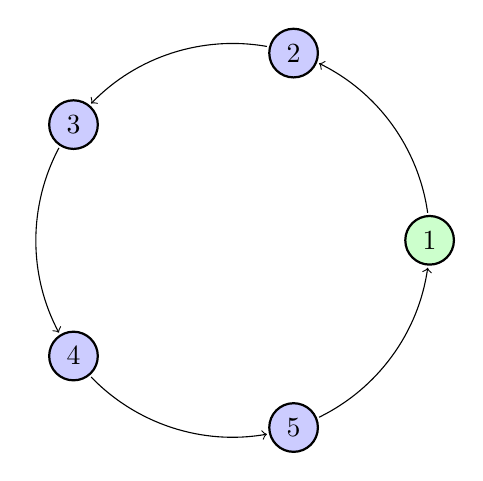
\begin{tikzpicture}[->,
	main node/.style={circle,draw,thick,fill=blue!20,minimum size=4mm},
	leader node/.style={circle,draw,thick,fill=green!20,minimum size=4mm}
]

	\def \n {5};
	\def \r {2.5cm};
	\def \m {8};

	\draw[->] (\m:\r) arc ({\m}:{360/\n -\m}:\r);

	\foreach \s in {2,...,\n} {
		\draw[->] ({360/\n * (\s-1) + \m}:\r) arc ({360/\n * (\s-1) + \m}:{360/\n * (\s) -\m}:\r);
		\node[main node] at ({360/\n * (\s-1)}:\r) {$\s$};
	}
	\node[leader node] at (0:\r) {1};
\end{tikzpicture}
\end{minipage}
\begin{minipage}{.5\textwidth}
\centering
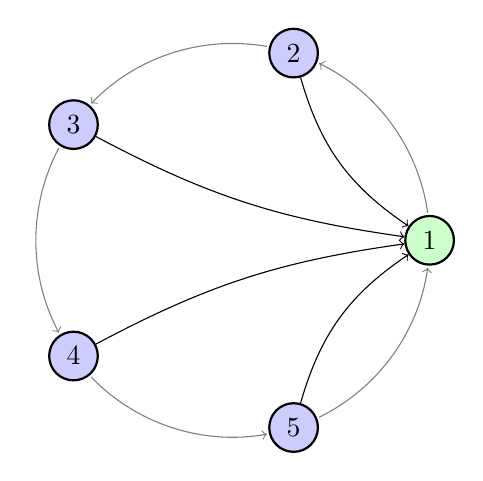
\begin{tikzpicture}[->,
	main node/.style={circle,draw,thick,fill=blue!20,minimum size=4mm},
	leader node/.style={circle,draw,thick,fill=green!20,minimum size=4mm}
]

	\def \n {5};
	\def \r {2.5cm};
	\def \m {8};

	\draw[->,gray] (\m:\r) arc ({\m}:{360/\n -\m}:\r);

	\foreach \s in {2,...,\n} {
		\draw[->,gray] ({360/\n * (\s-1) + \m}:\r) arc ({360/\n * (\s-1) + \m}:{360/\n * (\s) -\m}:\r);
		\node[main node] at ({360/\n * (\s-1)}:\r) (\s) {$\s$};
	}
	\node[leader node] at (0:\r) (L) {1};

	\draw[->] (2) to[bend right=20] (L);
	\draw[->] (3) to[bend right=10] (L);
	\draw[->] (4) to[bend left=10] (L);
	\draw[->] (5) to[bend left=20] (L);
\end{tikzpicture}
\end{minipage}
\end{figure}

La tolleranza ai guasti di tipo crash e' quindi stata progettata in
quest'ottica, ogni nodo potra' accorgersi del crash di un altro giocatore
all'istante (o al momento dell'interrogazione), e riconfigurera' l'ordine
dell'anello di sorta.

\begin{figure}[H]
	\begin{minipage}{0.45\textwidth}
		\centering
\begin{tikzpicture}[->,
	main node/.style={circle,draw,thick,fill=blue!20,minimum size=4mm},
	crashed node/.style={forbidden sign,draw,thick,fill=red!50,minimum size=4mm}
]

	\def \n {5};
	\def \r {2.5cm};
	\def \m {8};

	\draw[->,gray] (\m:\r) arc ({\m}:{360/\n -\m}:\r);

	\foreach \s in {2,...,\n} {
		\draw[->,gray] ({360/\n * (\s-1) + \m}:\r) arc ({360/\n * (\s-1) + \m}:{360/\n * (\s) -\m}:\r);
		\node[main node] at ({360/\n * (\s-1)}:\r) (\s) {$\s$};
	}
	\node[crashed node] at (0:\r) (L) {1};

	\draw[->] (2) to[bend right=20] (L);
	\draw[->] (3) to[bend right=10] (L);
	\draw[->] (4) to[bend left=10] (L);
	\draw[->] (5) to[bend left=20] (L);
\end{tikzpicture}
	\end{minipage}
	\begin{minipage}{0.45\textwidth}
		\centering
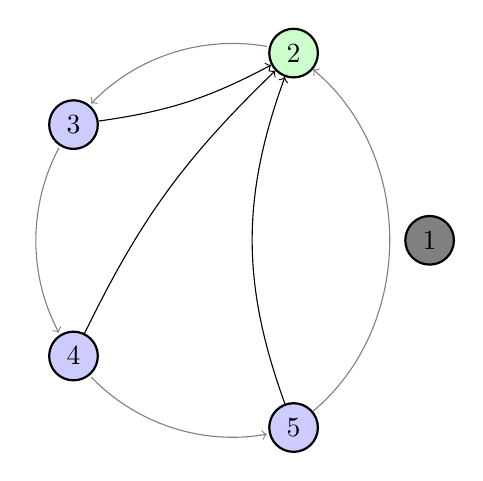
\begin{tikzpicture}[->,
	main node/.style={circle,draw,thick,fill=blue!20,minimum size=4mm},
	crashed node/.style={circle,draw,thick,fill=gray,minimum size=4mm},
	leader node/.style={circle,draw,thick,fill=green!20,minimum size=4mm}
]

	\def \n {5};
	\def \r {2.5cm};
	\def \m {8};


	\draw[->,gray] ({360/\n * (2-1) + \m}:\r) arc ({360/\n * (2-1) + \m}:{360/\n * (2) -\m}:\r);
	\node[leader node] at ({360/\n * (2-1)}:\r) (2) {$2$};
	\draw[->,gray] ({360/\n * (3-1) + \m}:\r) arc ({360/\n * (3-1) + \m}:{360/\n * (3) -\m}:\r);
	\node[main node] at ({360/\n * (3-1)}:\r) (3) {$3$};
	\draw[->,gray] ({360/\n * (4-1) + \m}:\r) arc ({360/\n * (4-1) + \m}:{360/\n * (4) -\m}:\r);
	\node[main node] at ({360/\n * (4-1)}:\r) (4) {$4$};
	\node[main node] at ({360/\n * (5-1)}:\r) (5) {$5$};

	\draw[->,gray] (5) to [bend right=50] (2);

	\node[crashed node] at (0:\r) (L) {1};
	\draw[->] (3) to[bend right=10] (2);
	\draw[->] (4) to[bend left=10] (2);
	\draw[->] (5) to[bend left=20] (2);
\end{tikzpicture}
	\end{minipage}
	\caption{Riconfigurazione dei client dovuta ad un crash}
\end{figure}
